% !TEX root = ../cube_einfty.tex

\section{An \texorpdfstring{${E_\infty}$}{E-infty}-structure on cubical chains} \label{s:action}

In this section we construct a natural $\M$-bialgebra structure on the chains of standard cubes.
These are determined by three natural linear maps satisfying the relations defining $\mathcal M$.
A Yoneda extension then provides the chains of any cubical set with a natural $\UM$-coalgebra structure.
We begin by recalling the basics of cubical topology.

\subsection{Cubical sets}

The objects of the \textit{cube category} $\cube$ are the sets $2^n = \{0, 1\}^n$ with $2^0 = \{0\}$ for $n \in \N$, and its morphisms are generated by the \textit{coface} and \textit{codegeneracy} maps
\begin{align*}
\delta_i^\varepsilon & = \mathrm{id}_{2^{i-1}} \times \delta^\varepsilon \times \mathrm{id}_{2^{n-1-i}} \colon 2^{n-1} \to 2^n, \\
\sigma_i & = \mathrm{id}_{2^{i-1}} \times \, \sigma \times \mathrm{id}_{2^{n-i}} \quad \colon 2^{n} \to 2^{n-1},
\end{align*}
where $\varepsilon \in \{0,1\}$ and the functors
\[
\begin{tikzcd} [column sep=16pt]
2^0 \arrow[r, bend left, "\delta^0"] \arrow[r, bend right, "\delta^1"'] & 2^1 \arrow[r, "\sigma"] & 2^0
\end{tikzcd}
\]
are defined by
\[
\delta^0(0) = 0, \qquad \delta^1(0) = 1, \qquad \sigma(0) = \sigma(1) = 0.
\]
We refer to \cite{grandis2003cubical} for a more leisure exposition and for variations on this definition.

We denote by $\cube_{\deg}(2^m, 2^n)$ the subset of morphism in $\cube(2^m, 2^n)$ of the form $\sigma_i \circ \tau$ with $\tau \in \cube(2^m, 2^{n+1})$.

The category of \textit{cubical sets} $\Fun(\cube^\op, \Set)$ is denoted by $\cSet$ and the representable cubical set $\yoneda(2^n)$ by $\cube^n$.
For any cubical set $X$ we write, as usual, $X_n$ instead of $X(2^n)$.

\subsection{Cubical topology}

Consider the topological $n$-cube
\begin{equation*}
\gcube^{n} = \big\{ (x_1, \dots, x_n) \mid x_i \in [0,1] \big\}.
\end{equation*}
The assignment $2^n \to \gcube^n$ defines a functor $\cube \to \Top$ with
\begin{align*}
\delta^\varepsilon_i(x_1, \dots, x_n) &= (x_1, \dots, x_i, \varepsilon, x_{i+1}, \dots x_n), \\
\sigma_i(x_1,\dots,x_n) &= (x_1, \dots, \widehat{x}_i, \dots, x_n).
\end{align*}
Its Yoneda extension is known as \textit{geometric realization}.
It has a right adjoint $\cSing \colon \Top \to \cSet$ referred to as the \textit{cubical singular complex} satisfying
\[
\cSing(\fZ)_n = \Top(\gcube^n, \fZ)
\]
for any topological space $\fZ$.

\subsection{Cubical chains}

The functor of (\textit{normalized}) \textit{chains} $\chains \colon \cSet \to \Ch$ is the Yoneda extension of the functor $\cube \to \Ch$ defined next.
It assigns to an object $2^n$ the chain complex having in degree $m$ the module
\[
\frac{\k\{\cube(2^m, 2^n)\}}{\k\{\cube_{\deg}(2^m, 2^n)\}}
\]
and differential induced by
\[
\bd (\id_{2^n}) = \sum_{i=1}^{n} \ (-1)^i \
\big(\delta_i^1 - \delta_i^0 \big).
\]
To a morphism $\tau \colon 2^n \to 2^{n'}$ it assigns the chain map
\[
\begin{tikzcd}[row sep=-3pt, column sep=normal,
/tikz/column 1/.append style={anchor=base east},
/tikz/column 2/.append style={anchor=base west}]
\chains(\cube^n)_m \arrow[r] & \chains(\cube^{n'})_m \\
\big( 2^m \to 2^n \big) \arrow[r, mapsto] & \big( 2^m \to 2^n \stackrel{\tau}{\to} 2^{n'} \big).
\end{tikzcd}
\]
The chain complex $\chains(\cube^n)$ is isomorphic to both: $\chains(\cube^1)^{\ot n}$ and the cellular chains on the topological $n$-cube with its standard CW structure $\gchains(\gcube^n)$.
We use the isomorphism $\chains(\cube^n) \cong \gchains(\gcube^1)^{\ot n}$ when denoting the elements in the basis of $\chains(\cube^n)$ by $x_1 \ot \dotsb \ot x_n$ with $x_i \in \{[0], [0,1], [1]\}$.

For a topological space $\fZ$, the chain complex $\chains(\cSing \fZ)$ is referred to as the \textit{cubical singular chains} of $\fZ$.

\subsection{Serre coalgebra} \label{ss:serre coalgebra}

We now recall the natural (counital and coassociative) coalgebra structure on cubical chains studied by Cartan and Serre, inducing the cup product in the cohomology of cubical sets.

Using a Yoneda extension, it suffices to equip the chains on standard cubes with a natural coalgebra structure.
For any $n \in \N$, define $\epsilon \colon \chains(\cube^n) \to \k$ by
\[
\epsilon \left( x_1 \ot \dotsb \ot x_d \right) = \epsilon(x_1) \dotsm \epsilon(x_n),
\]
where
\[
\epsilon([0]) = \epsilon([1]) = 1, \qquad \epsilon([0, 1]) = 0,
\]
and $\Delta \colon \chains(\cube^n) \to \chains(\cube^n)^{\ot 2}$ by
\[
\Delta (x_1 \ot \dotsb \ot x_n) =
\sum \pm \left( x_1^{(1)} \ot \dotsb \ot x_n^{(1)} \right) \ot
\left( x_1^{(2)} \ot \dotsb \ot x_n^{(2)} \right),
\]
where the sign is determined using the Koszul convention, and we are using Sweedler's notation
\[
\Delta(x_i) = \sum x_i^{(1)} \ot x_i^{(2)}
\]
for the chain map $\Delta \colon \chains(\cube^1) \to \chains(\cube^1)^{\ot 2}$ defined by
\[
\Delta([0]) = [0] \ot [0], \quad \Delta([1]) = [1] \ot [1], \quad \Delta([0,1]) = [0] \ot [0,1] + [0,1] \ot [1].
\]

We remark that, using the canonical isomorphism $\chains(\cube^n) \cong \chains(\cube^1)^{\ot n}$, the coproduct $\Delta$ can be described as the composition
\[
\begin{tikzcd}
\chains(\cube^1)^{\ot n} \arrow[r, "\Delta^{\ot n}"] & \left( \chains(\cube^1)^{\ot 2} \right)^{\ot n} \arrow[r, "\pi"] & \left( \chains(\cube^1)^{\ot n} \right)^{\ot 2}
\end{tikzcd}
\]
where $\pi$ is the shuffle permutation of tensor factors placing those in odd positions first.

\subsection{Degree 1 product}

For $n \in \mathbb{N}$ define the \textit{product} $\ast  \colon \chains(\square^n)^{\ot 2} \to \chains(\square^n)$ by
\begin{multline*}
(x_1 \ot \dotsb \ot x_n) \ast (y_1 \ot \dotsb \ot y_n) = \\
(-1)^{|x|} \sum_{i=1}^n x_{<i}\, \epsilon(y_{<i}) \ot x_i \ast y_i \ot \epsilon(x_{>i}) \, y_{>i},
\end{multline*}
where
\begin{align*}
x_{<i} & = x_1 \ot \dotsb \ot x_{i-1}, &
y_{<i} & = y_1 \ot \dotsb \ot y_{i-1}, \\
x_{>i} & = x_{i+1} \ot \dotsb \ot x_n, &
y_{>i} & = y_{i+1} \ot \dotsb \ot y_n,
\end{align*}
with the convention
\[
x_{<1} = y_{<1} = x_{>n} = y_{>n} = 1 \in \Z,
\]
and the only non-zero values of $x_i \ast y_i$ are
\[
\ast([0] \ot [1]) = [0, 1], \qquad  \ast([1] \ot [0]) = -[0, 1].
\]

\subsection{$\M$-bialgebra on representable cubical sets}

\begin{lemma} \label{l:cubical chain bialgebra}
	The assignment
	\[
	\counit \mapsto \epsilon, \quad \coproduct \mapsto \Delta, \quad \product \mapsto \ast,
	\]
	induces a natural $\mathcal M$-bialgebra structure on $\chains(\square^n)$ for every $n \in \mathbb{N}$.
\end{lemma}

\begin{proof}
	We need to show that this assignment is compatible with the relations
	\[
	\productcounit = 0, \qquad
	\leftcounitality = 0, \qquad
	\rightcounitality = 0,
	\]
	and
	\[
	\bd\ \counit = 0, \qquad
	\bd\ \coproduct = 0, \qquad
	\bd\ \product = \ \boundary\,.
	\]
	For the rest of this proof let us consider two basis elements of $\chains(\square^n)$
	\begin{align*}
		x = x_1 \ot \dotsb \ot x_n
		\qquad \text{ and } \qquad
		y = y_1 \ot \dotsb \ot y_n.
	\end{align*}
	Since the degree of $\ast$ is $1$ and $\epsilon([0,1]) = 0$, we can verify the first relation easily:
	\begin{align*}
		\varepsilon(x \ast y) & =
		\sum (-1)^{|x|} \epsilon(y_{<i}) \epsilon(x_{<i}) \ot \epsilon(x_i \ast y_i) \ot \epsilon(x_{>i}) \epsilon(y_{>i}) = 0.
	\end{align*}
	For the second relation we want to show that $(\epsilon \ot \id) \circ \Delta = \id$.
	Since
	\begin{gather*}
		(\epsilon \ot \id) \circ \Delta([0]) = \epsilon([0]) \ot [0] = [0], \\
		(\epsilon \ot \id) \circ \Delta([1]) = \epsilon([1]) \ot [1] = [1], \\
		(\epsilon \ot \id) \circ \Delta([0, 1]) = \epsilon([0]) \ot [0, 1] + \epsilon([0, 1]) \ot [1] = [0,1],
	\end{gather*}
	we have
	\begin{multline*}
		(\epsilon \ot \id) \circ \Delta (x_1 \ot \dotsb \ot x_n) = \\
		\sum \pm \left( \epsilon \big(x_1^{(1)}\big) \ot \dotsb \ot \epsilon\big(x_n^{(1)}\big) \right) \ot
		\left( x_1^{(2)} \ot \dotsb \ot x_n^{(2)} \right) \\ =
		x_1 \ot \dotsb \ot x_n,
	\end{multline*}
	where the sign is obtained by noticing that the only non-zero term occurs when each factor $x_i^{(0)}$ is of degree $0$.
	The third relation is verified analogously.
	The fourth and fifth are precisely the well known facts that $\epsilon$ and $\Delta$ are chain maps.
	To verify the sixth and final relation we need to show that
	\[
	\bd (x \ast y)\ +\ \bd x \ast y\ +\ (-1)^{|x|}x \ast \bd y\ =\ \epsilon(x) y \ -\ \epsilon(y) x.
	\]
	We have
	\[
	x \ast y = \sum (-1)^{|x|} x_{<i} \, \epsilon(y_{<i}) \ot x_i \ast y_i \ot \epsilon(x_{>i})\, y_{>i}
	\]
	and
	\begin{align*}
		\bd(x \ast y) & =
		\sum (-1)^{|x|} \, \bd x_{<i}\, \epsilon(y_{<i}) \ot x_i \ast y_i \ot \epsilon(x_{>i})\, y_{>i} \\ & +
		\sum (-1)^{|x|+|x_{<i}|} \, x_{<i}\, \epsilon(y_{<i}) \ot \bd (x_i \ast y_i) \ot \epsilon(x_{>i}) \, y_{>i} \\ & -
		\sum (-1)^{|x|+|x_{<i}|} \, x_{<i}\, \epsilon(y_{<i}) \ot x_i \ast y_i \ot \epsilon(x_{>i})\, \bd y_{>i}.
	\end{align*}
	Since $|x| = |x_{<i}| + |x_i| + |x_{>i}|$ and $\epsilon(x_{>i}) \neq 0 \Leftrightarrow |x_{>i}| = 0$ as well as $\bd(x_i \ast y_i) \neq 0 \Rightarrow |x_i| = 0$
%	\[
%	|x| = |x_{<i}| + |x_i| + |x_{>i}|, \quad \epsilon(x_{>i}) \neq 0 \Leftrightarrow |x_{>i}| = 0, \quad \bd(x_i \ast y_i) \neq 0 \Rightarrow |x_i| = 0,
%	\]
	we have
	\begin{equation} \label{e:boundary of product 1}
		\begin{split}
			\bd(x \ast y) & =
			\sum (-1)^{|x|} \, \bd x_{<i}\, \epsilon(y_{<i}) \ot x_i \ast y_i \ot \epsilon(x_{>i})\, y_{>i} \\ & +
			\sum x_{<i} \, \epsilon(y_{<i}) \ot \bd (x_i \ast y_i) \ot \epsilon(x_{>i})\, y_{>i} \\ & -
			\sum x_{<i} \, \epsilon(y_{<i}) \ot x_i \ast y_i \ot \epsilon(x_{>i})\, \bd y_{>i}.
		\end{split}
	\end{equation}
	We also have
	\begin{align*}
		\bd x \ast y & =
		\sum (-1)^{|x|-1} \, \bd x_{<i}\, \epsilon(y_{<i}) \ot x_i \ast y_i \ot \epsilon(x_{>i}) \, y_{>i} \\ & +
		\sum (-1)^{|x|-1+|x_{<i}|} \, x_{<i}\, \epsilon(y_{<i}) \ot \bd x_i \ast y_i \ot \epsilon(x_{>i}) \, y_{>i} \\ & +
		\sum (-1)^{|x|-1+|x_{<i}|} \, x_{<i}\, \epsilon(y_{<i}) \ot x_i \ast y_i \ot \epsilon(\bd x_{>i}) \, y_{>i}.
	\end{align*}
	Since
	\[
	\epsilon(\bd x_{>i}) = 0, \quad \bd x_i \neq 0 \Leftrightarrow |x_i| = 1,
	\]
	we have
	\begin{equation} \label{e:boundary of product 2}
		\begin{split}
			\bd x \ast y & =
			\sum (-1)^{|x|-1} \, \bd x_{<i}\, \epsilon(y_{<i}) \ot x_i \ast y_i \ot \epsilon(x_{>i})\, y_{>i} \\ & +
			\sum x_{<i}\, \epsilon(y_{<i}) \ot \bd x_i \ast y_i \ot \epsilon(x_{>i})\, y_{>i}.
		\end{split}
	\end{equation}
	We also have
	\begin{align*}
		(-1)^{|x|} \, x \ast \bd y & =
		\sum x_{<i} \, \epsilon(\bd y_{<i}) \ot x_i \ast y_i \ot \epsilon(x_{>i})\, y_{>i} \\ & +
		\sum (-1)^{|y_{<i}|} \, x_{<i}\, \epsilon(y_{<i}) \ot x_i \ast \bd y_i \ot \epsilon(x_{>i}) \, y_{>i} \\ & +
		\sum (-1)^{|y_{<i}| + |y_i|} \, x_{<i}\, \epsilon(y_{<i}) \ot x_i \ast y_i \ot \epsilon(x_{>i}) \, \bd y_{>i},
	\end{align*}
	which is equivalent to
	\begin{equation} \label{e:boundary of product 3}
		\begin{split}
			(-1)^{|x|} \, x \ast \bd y & =
			\sum x_{<i} \, \epsilon(y_{<i}) \ot x_i \ast \bd y_i \ot \epsilon(x_{>i})\, y_{>i} \\ & +
			\sum x_{<i}\, \epsilon(y_{<i}) \ot x_i \ast y_i \ot \epsilon(x_{>i})\, \bd y_{>i}.
		\end{split}
	\end{equation}
	Putting identities \eqref{e:boundary of product 1}, \eqref{e:boundary of product 2} and \eqref{e:boundary of product 3} together, we get
	\begin{multline*}
		\bd (x \ot y) \ +\ \bd x \ast y\ +\, (-1)^{|x|}x \ast \bd y \\
		= \sum \epsilon(y_{<i})\, x_{<i} \ot \big(\bd(x_i \ast y_i) + \bd x_i \ast y_i + x_i \ast \bd y_i\big) \ot \epsilon(x_{>i})\, y_{>i}.
	\end{multline*}
	Since
	\begin{align*}
		\bd(x_i \ast y_i)\ +\ \bd x_i \ast y_i\ +\ x_i \ast \bd y_i =
		\epsilon(x_i)y_i\ -\ \epsilon(y_i)x_i,
	\end{align*}
	we have
	\begin{multline*}
		\bd (x \ast y) \ +\ \bd x \ast y\ +\ (-1)^{|x|}x \ast \bd y  = \\
		\sum \epsilon(y_{<i}) \, x_{<i} \ot \epsilon(x_{\geq i}) y_{\geq i}\ -\
		\epsilon(y_{\leq i}) \, x_{\leq i} \ot \epsilon(x_{>i}) y_{>i} \\ =
		\epsilon(x)y - \epsilon(y)x,
	\end{multline*}
	as desired, where the last equality follows from a telescopic sum argument.
\end{proof}

\subsection{$\texorpdfstring{E_\infty}{E-infty}$-coalgebra on cubical chains}

\cref{l:cubical chain bialgebra} defines a functor from the cube category to that of $\Med$-bialgebras.
This category is not cocomplete so we do not expect to have an $\Med$-bialgebra structure on arbitrary cubical sets.
For example, consider the chains on the cubical set $X$ whose only non-degenerate simplices are $v, w \in X_0$.
By degree reasons $v \ast w = 0$ for any degree 1 product $\ast$ in $\chains(X)$.
The third relation in $\Med$ would then imply the contradiction $0 = w-v$.
Nevertheless, categories of coalgebras over operads are cocomplete and we have the following.

\begin{theorem} \label{t:lift to e infinity coalgebras}
	The Yoneda extension of the composition of the functor $\cube \to \biAlg_{\M}$ defined in \cref{l:cubical chain bialgebra} with the forgetful functor $\biAlg_{\M} \to \coAlg_{\UM}$ endows the chains of a cubical set with a natural $E_\infty$-coalgebra extension of the Serre coalgebra structure.
\end{theorem}

Using linear duality, the same argument can be employed to define a natural $E_\infty$-algebra structure on cubical cochains.
Explicitly, let $X$ be a cubical set, $x$ a simplex and $f \colon \chains(\cube^n) \to \chains(X)$ a chain map sending $\id_{2^n}$ to $x$.
The image $\gamma$ in $\Hom(\chains(\cube^n), \chains(\cube^n)^{\ot r})$ of a basis element $\Gamma$ in $\UM(r)$ is either $\varepsilon$ or a composition of $\Delta$, permutations of factors, and $\ast$.
For any $\alpha_1, \dots, \alpha_r \in \cochains(X)$ the action of $\Gamma$ on these is given by
\[
\Gamma(\alpha_1, \dots, \alpha_r)(x) = (\alpha_1 \ot \dotsb \ot \alpha_r) \circ f^{\ot r} \circ \gamma(\id_{2^n}).
\]

\subsection{Cohomology operations}

Steenrod introduced in \cite{steenrod1947products} operations on the mod~2 cohomology of spaces via an explicit construction in the simplicial context of natural linear maps $\Delta_i$ satisfying up to signs the following homological relations
\begin{equation} \label{e:cupi homological relations}
\bd \circ \Delta_i + \Delta_i \circ \bd = (1 + T) \Delta_{i-1}
\end{equation}
with the convention $\Delta_{-1} = 0$.
These maps, referred to as (simplicial) cup-$i$ coproducts, are fundamental combinatorially, admitting an axiomatic characterization \cite{medina2022axiomatic} and defining, for example, the nerve of $n$-categories as introduced by Street \cite{street1987orientals, medina2020globular}.

In the cubical case, cup-$i$ coproducts were defined in \cite{kadeishvili1999coproducts} and \cite{pilarczyk2016cubical}.
It is unclear if these are equivalent.
The formulas used by these authors are analogous to those introduced in \cite{medina2021fast_sq} for the simplicial case, a dual yet equivalent version of Steenrod's original description.
By the same methods used in \cite{medina2020globular}, these formulas define a cubical nerve for higher categories, but it remains unclear if either agrees with the one defined by the generalized Gray tensor product.

A new description of cubical cup-$i$ coproducts can be deduced from our $E_\infty$-structure on cubical chains by considering the action of the elements depicted in \cref{f:cup-i}.
\begin{figure}
	\centering
	\boxed{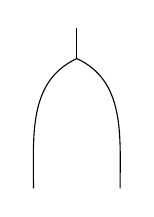
\begin{tikzpicture}[scale=.55]
			\draw (1,3.7) to (1,3);

			\draw (1,3) to [out=205, in=90] (0,0);
			\draw (1,3) to [out=-25, in=90] (2,0);

		\end{tikzpicture}\hspace*{1cm}
		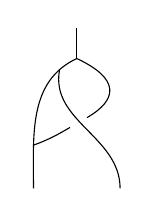
\begin{tikzpicture}[scale=.55]
			\draw (1,3.7) to (1,3);

			\draw (1,3) to [out=205, in=90] (0,0);

			\draw [shorten >= 0cm] (.6,2.73) to [out=-100, in=90] (2,0);

			\draw [shorten >= .15cm] (1,3) to [out=-25, in=30, distance=1.1cm] (1,1.5);
			\draw [shorten <= .1cm] (1,1.5) to [out=210, in=20] (0,1);

		\end{tikzpicture}\hspace*{1cm}
		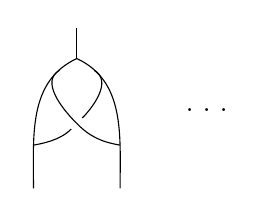
\begin{tikzpicture}[scale=.55]
			\draw (1,3.7) to (1,3);

			\draw (1,3) to [out=205, in=90] (0,0);
			\draw (1,3) to [out=-25, in=90] (2,0);

			\draw [shorten >= 0cm] (.6,2.73) to [out=210, in=135] (1,1.5);
			\draw [shorten <= 0cm] (1,1.5) to [out=-45, in=170] (2,1);

			\draw [shorten >= .1cm] (1.4,2.73) to [out=-30, in=45] (1,1.5);
			\draw [shorten <= .1cm] (1,1.5) to [out=-135, in=10] (0,1);

			\node at (4,1.8){.\ .\ .};
	\end{tikzpicture}}
	\caption{Elements in $\UM$ defining cubical cup-$i$ coproducts.}
	\label{f:cup-i}
\end{figure}
These recursively define:
\begin{equation} \label{e:prop cup-i}
	\begin{split}
		& \Delta_0 = \Delta, \\
		& \Delta_i =
		(\ast \ot \id) \circ (\id \ot (12) \Delta_{i-1}) \circ \Delta.
	\end{split}
\end{equation}
It is not known if these agree with either of the previous constructions, pointing to the value of an axiomatic characterization as it exists in the simplicial case, where all known constructions agree.

Cup-$i$ coproducts represent at the cochain level Steenrod squares
\[
\begin{tikzcd} [column sep=small, row sep=0]
	Sq^k \colon &[-20] H^{-n} \arrow[r] & H^{-n-k} \\ &
	{[\alpha]} \arrow[r, mapsto] & \big[ (\alpha \ot \alpha) \Delta_i \big]
\end{tikzcd}
\]
which are primary operations in mod~2 cohomology.
To obtain secondary cohomology operations one studies the cohomological relations these operations satisfy, for example the Cartan and Adem relations \cite{steenrod1962cohomology}.
To do this at the cubical chain level, as it was done in \cite{medina2020cartan,medina2021adem} for the simplicial case, the operadic viewpoint is important, so our $E_\infty$-structure on cubical cochains invites the construction of cochain representatives for secondary operations in the cubical case.

For an odd $p$, Steenrod also introduced operations on the mod $p$ cohomology of spaces using the homology of symmetric groups \cite{steenrod1952reduced, steenrod1953cyclic}.
Using the operadic framework of May \cite{may1970general}, we described in \cite{medina2021may_st} elements in $\UM$ representing multicooperations defining Steenrod operations at any prime.
In particular, as proven in this work, these so-called cup-$(p,i)$ products are defined on cubical cochains and are expressible, similarly to \cref{e:prop cup-i}, in terms of $\Delta$, the permutations of factors, and $\ast$.
The aforementioned construction of cubical cup-$(p,i)$ coproducts has been implemented in the computer algebra system \href{https://comch.readthedocs.io/en/latest/}{\texttt{ComCH}} \cite{medina2021comch}.
